%
%
%   LQuiz 12 : 2022--03--03 (R)
%
%

\section{Exercise}

% Reference : SHW
% Graphing tool : https://www.desmos.com/calculator

(4 pt) Let $f : \reals \rightarrow \reals$ be the function whose rule of assignment is
\begin{align*}
f(x)
=
x^{2} - 2 x + 2
\end{align*}
This exercise explores the area under the graph of $f$ from $x = 0$ to $x = 3$, that is,
\begin{align}
\int_{0}^{3} f(x) \spaceIntd \intd x%
\label{eq : LQ12 Definite Integral}
\end{align}



\begin{enumerate}[label=(\alph*)]
\item\label{itm : LQ12a} (2 pt) The function $f$ is graphed below, twice. Draw a lower sum and an upper sum, on separate graphs, each with three subintervals of length $1$, for the definite integral in \eqref{eq : LQ12 Definite Integral}. Compute the values $L$ and $U$, respectively, of these two sums.
\begin{center}
%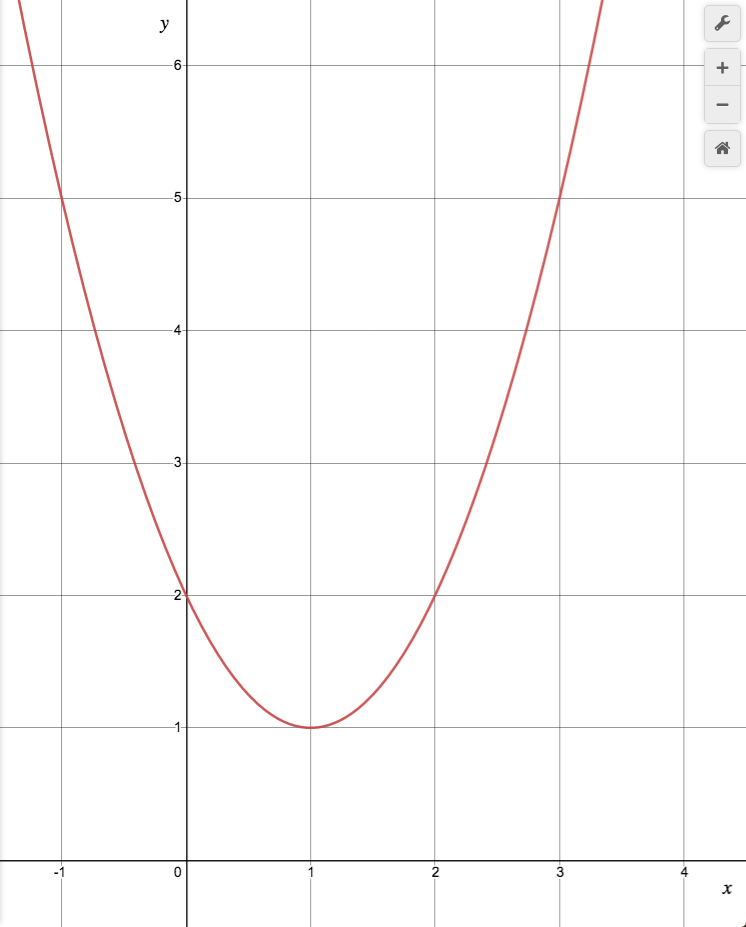
\includegraphics[scale=0.15]{\filePathGraphics/LQ12_Graph.png}% Activate for quiz.
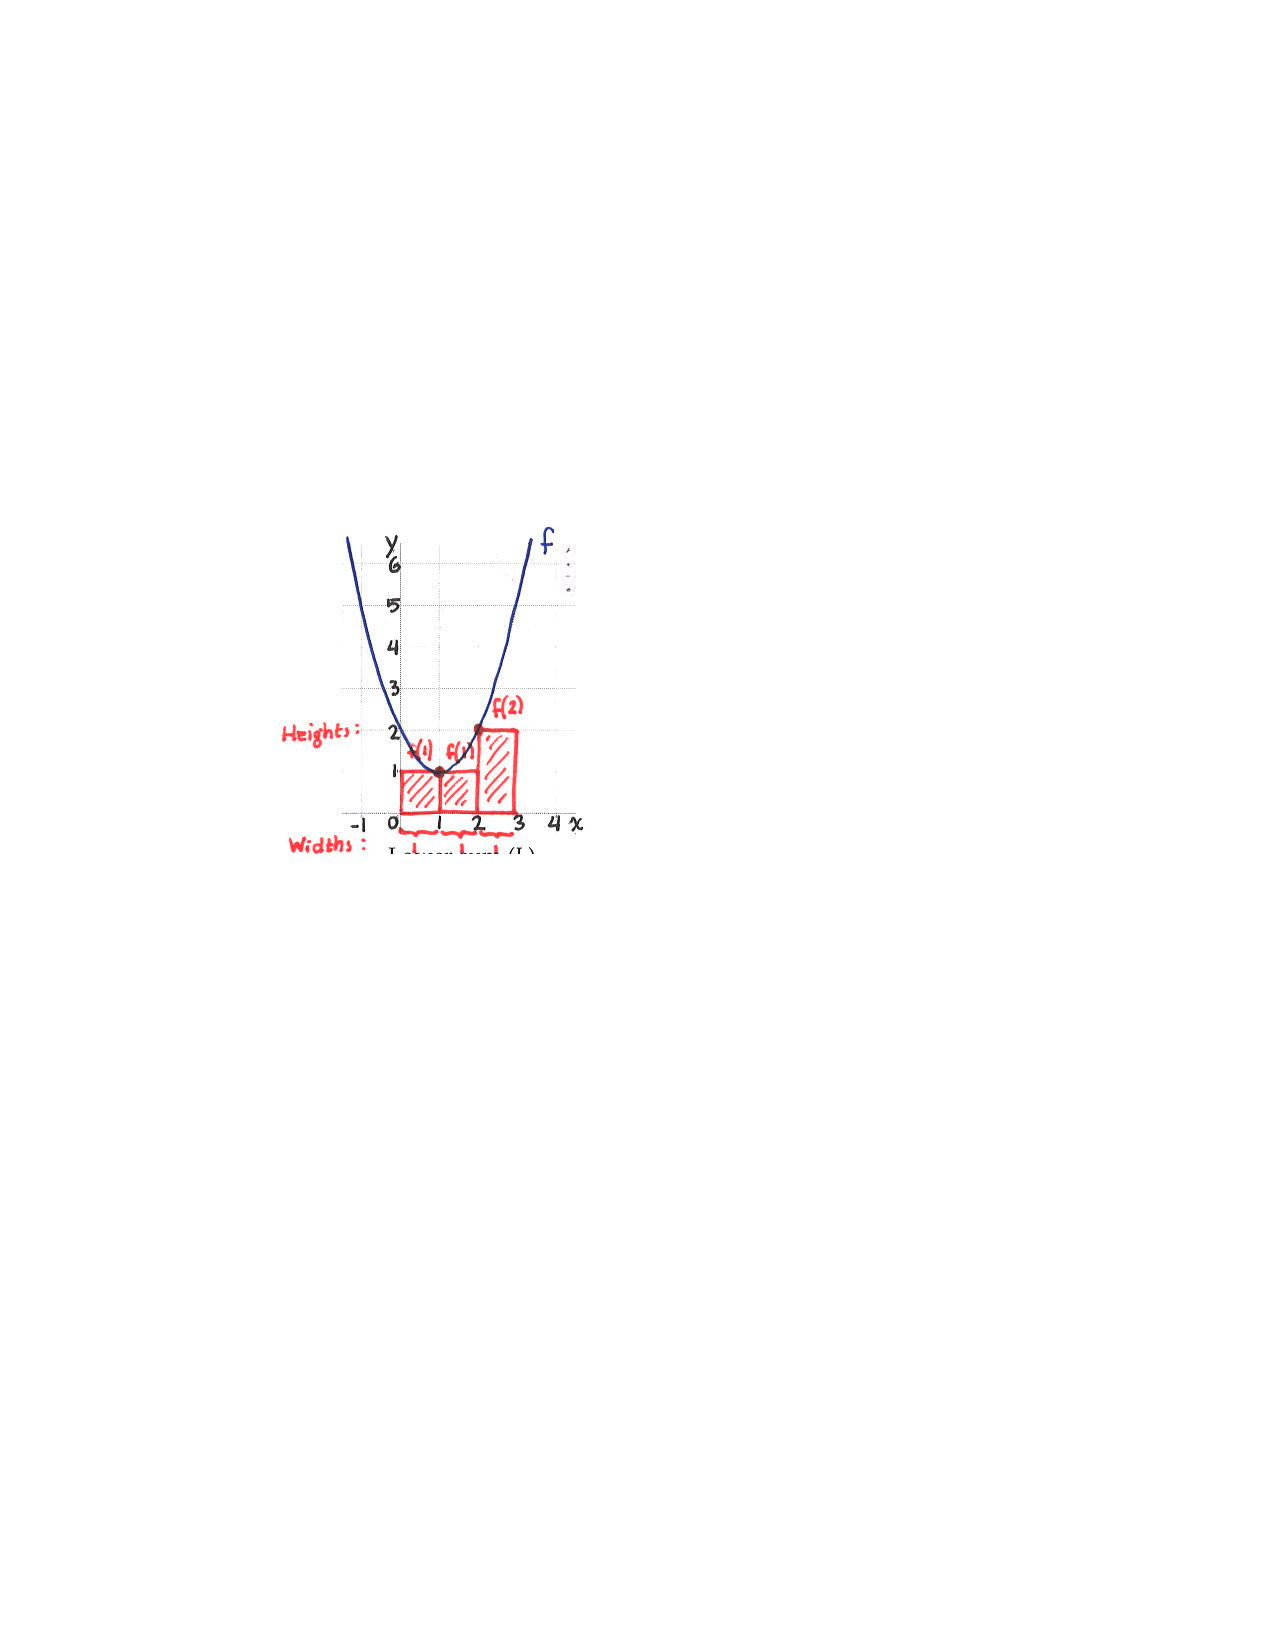
\includegraphics[scale=0.8]{\filePathGraphics/LQ12_Graph_Lower.pdf}% Activate for solutions.
\hspace{1in}
%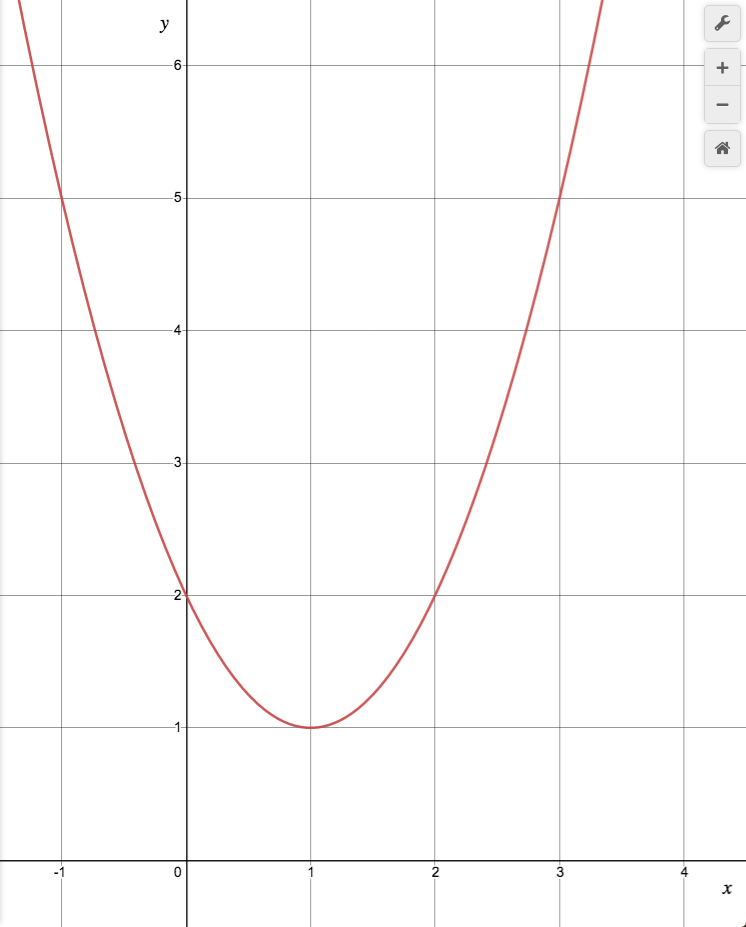
\includegraphics[scale=0.15]{\filePathGraphics/LQ12_Graph.png}% Activate for quiz.
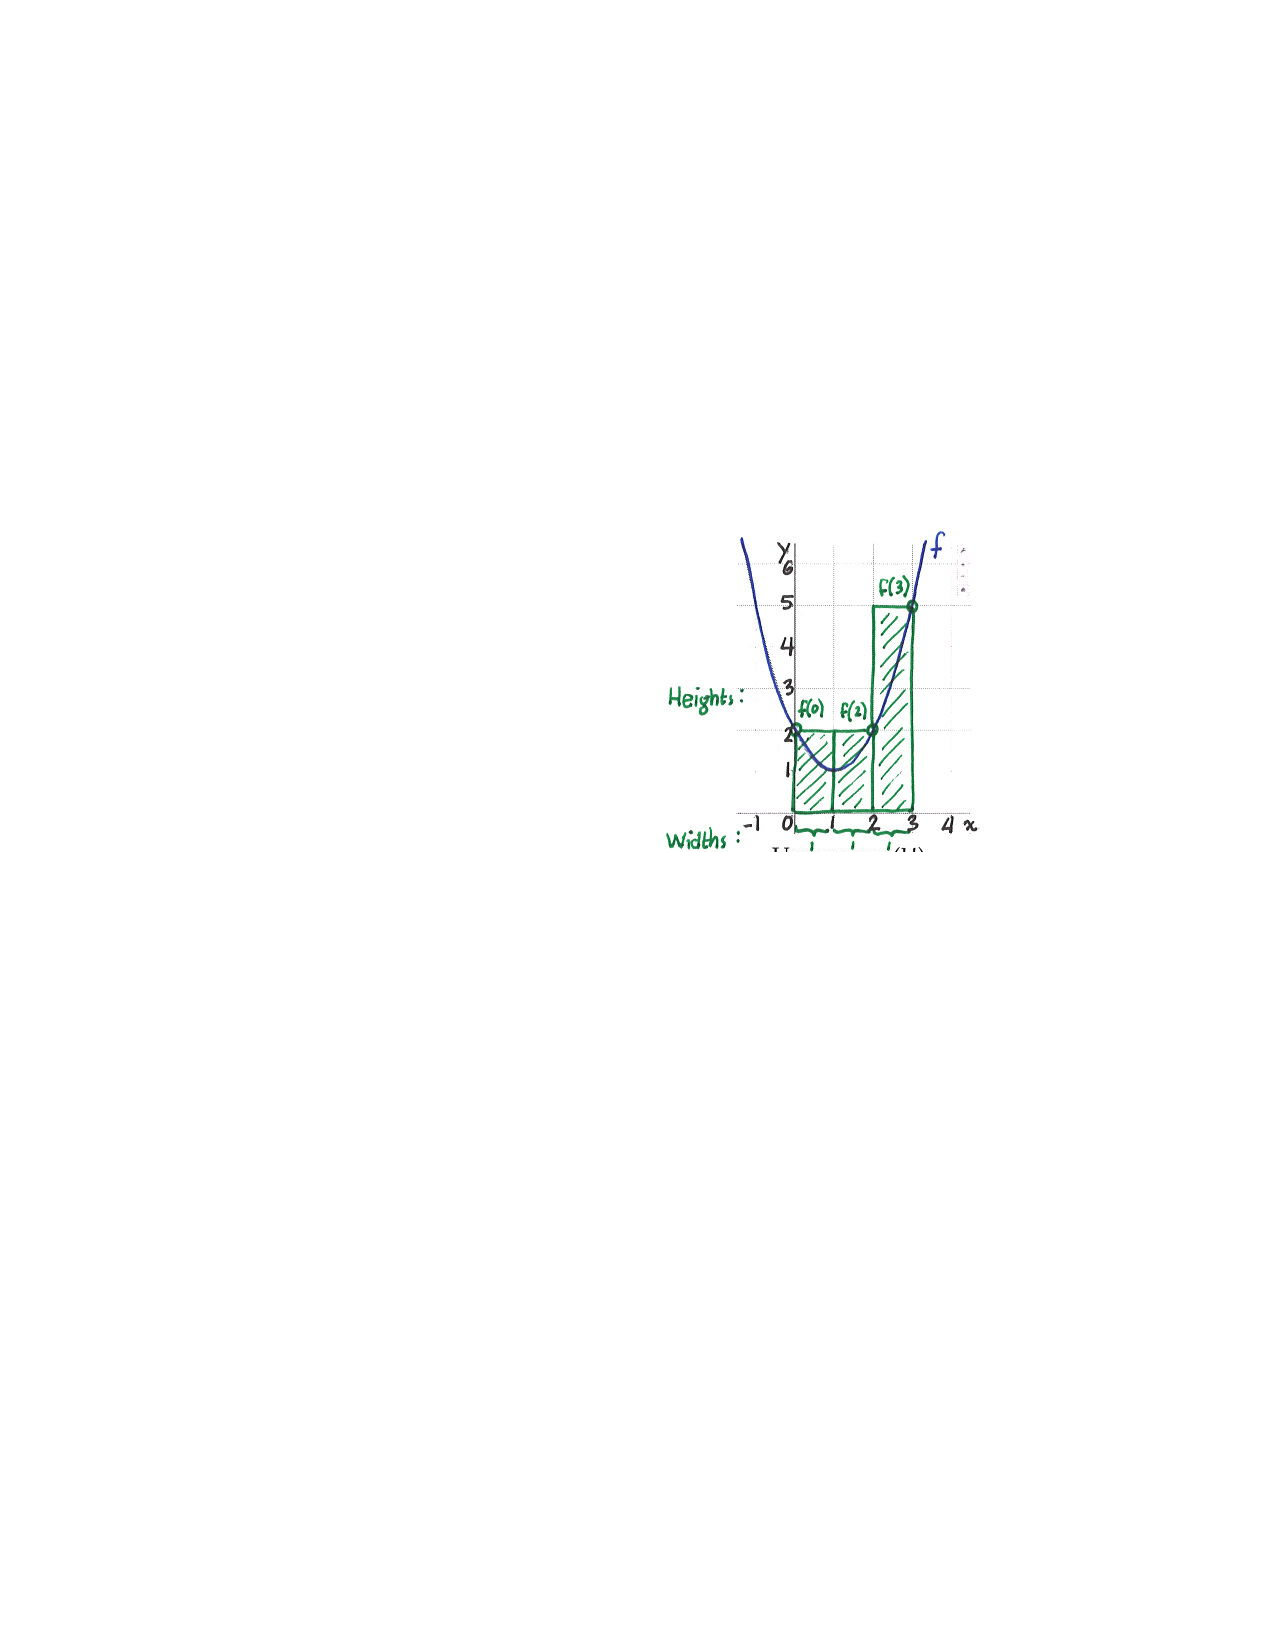
\includegraphics[scale=0.8]{\filePathGraphics/LQ12_Graph_Upper.pdf}% Activate for solutions.
\\
Lower sum ($L$)
\hspace{1.5in}
Upper sum ($U$)
\end{center}
\end{enumerate}

\spaceSolution{1in}{% Begin solution.
The lower sum $L$ has value (area) $4$. More precisely,
\begin{align*}
L
=
f(1) \cdot 1 + f(1) \cdot 1 + f(2) \cdot 1
=
1 \cdot 1 + 1 \cdot 1 + 2 \cdot 1
=
4
\end{align*}
The upper sum $U$ has value (area) $9$. More precisely,
\begin{align*}
U
=
f(0) \cdot 1 + f(2) \cdot 1 + f(3) \cdot 1
=
2 \cdot 1 + 2 \cdot 1 + 5 \cdot 1
=
9
\end{align*}}% End solution.



\begin{enumerate}[resume,label=(\alph*)]
\item\label{itm : LQ12b} (2 pt) Find an antiderivative $F(x)$ of $f(x)$. Compute the difference $F(3) - F(0)$. Compare the result to the lower and upper sum you computed in part \ref{itm : LQ12a}.
\end{enumerate}

\spaceSolution{2in}{% Begin solution.
The function $F : \reals \rightarrow \reals$ given by
\begin{align*}
F(x)
=
\frac{1}{3} x^{3} - x^{2} + 2 x
\end{align*}
is an antiderivative of $f(x)$, as we can confirm by differentiating (that is, $F'(x) = f(x)$). We compute
\begin{align*}
F(3)
=
6
&&
F(0)
=
0
&&
F(3) - F(0)
=
6 - 0
=
6
\end{align*}
This value lies between the lower sum $L$ and upper sum $U$ we computed in part \ref{itm : LQ12a}:
\begin{align*}
L
=
4
\leq
F(3) - F(0)
\leq
9
=
U
\end{align*}
N.B. This difference $F(3) - F(0)$ is the exact area under the graph of $f$ from $x = 0$ to $x = 3$.}% End solution.